\documentclass[12pt,a4paper]{article}
\usepackage[utf8]{inputenc} % sempre salve seus arquivos como UTF8
\usepackage[T1]{fontenc}
\usepackage[english]{babel}

\usepackage[left=2.5cm,right=2cm,top=2cm,bottom=2.5cm]{geometry}
\usepackage{amsmath}
\usepackage{amsthm}
\usepackage{amsfonts}

\usepackage{graphicx}
\usepackage{algorithm}
\usepackage{color}
\usepackage[noend]{algpseudocode}
\usepackage{mathtools}
\usepackage{subfig}
\usepackage{diagbox}

% load times font
\usepackage{mathptmx}
\usepackage[scaled=.90]{helvet}
\usepackage{courier}

% comandos
\newcommand{\mdc}[1]{\mathrm{mdc}(#1)}

\DeclarePairedDelimiter\ceil{\lceil}{\rceil}
\DeclarePairedDelimiter\floor{\lfloor}{\rfloor}

% Foot without marker
\newcommand\blfootnote[1]{%
	\begingroup
	\renewcommand\thefootnote{}\footnote{#1}%
	\addtocounter{footnote}{-1}%
	\endgroup
}

\title{MO446 -- Introduction to Computer Vision  \\ Project 1}
\author{Breno Leite  \\ Guilherme Leite}
\date{28/08/2017}

\begin{document}

\maketitle
\blfootnote{\textit{\textbf{Important note:} The borders seen in the figures are not part of the image, they are figurative information about the starting and ending points of the image. Moreover, all the image scales in this report were changed in order to make the text more readable.}} \\

%% ---------------- Starts here --------------------------------

\textbf{\LARGE Input Images}\\

Throughout this project some images were used as input to test the algorithms. Figure \ref{fig:p1-1-0} was used as input for the pyramids exercises \textbf{2.1, 2.2, 2.3} and \textbf{3.1}, its dimensions are 400x300 and it is a colored image. \\

\begin{figure}[!h]
	\centering
	{%
		\setlength{\fboxsep}{1pt}%
		\setlength{\fboxrule}{1pt}%
		\fbox{
\includegraphics[scale=1]{input/p1-1-0}}%
	}%
	\caption{Input image for pyramids and Fourier transform exercises. (\textbf{p1-1-0})}
	\label{fig:p1-1-0}
\end{figure}

\newpage

Images in Figure \ref{fig:blending} are used for the blending exercises (\textbf{2.4} and \textbf{3.2}), their dimensions is 540x392. Note that the images are slightly rotated, this will affect some results which comes from the image and not by any error on the process itself.\\

\begin{figure}[!h]
	\centering
	\subfloat[(\textbf{p1-2-4-0})]{
		{
			\setlength{\fboxsep}{1pt}
			\setlength{\fboxrule}{1pt}
			\fbox{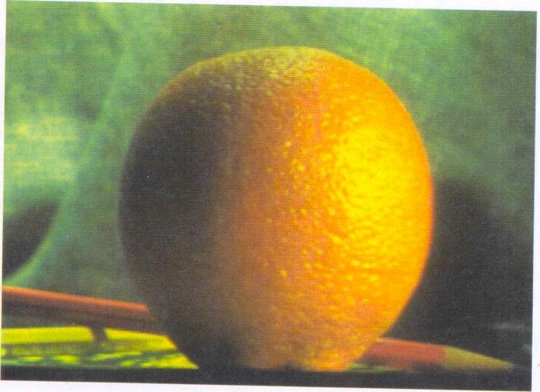
\includegraphics[scale=0.5]{input/p1-2-4-0}}
		}
	}
	\quad
	\subfloat[(\textbf{p1-2-4-1})]{
		{
			\setlength{\fboxsep}{1pt}
			\setlength{\fboxrule}{1pt}
			\fbox{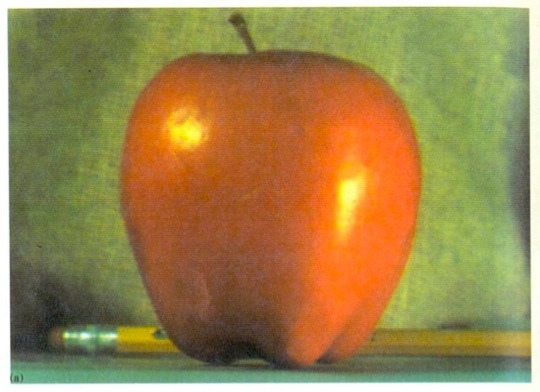
\includegraphics[scale=0.5]{input/p1-2-4-1}}
		}
	}
	\quad
	\subfloat[(\textbf{p1-2-4-2})]{
		{
			\setlength{\fboxsep}{1pt}
			\setlength{\fboxrule}{1pt}
			\fbox{
\includegraphics[scale=0.25]{input/p1-2-4-2}}
		}
	}
	\caption{Images (a), (b) and (c) used for the blending operations.}
	\label{fig:blending}
\end{figure}
	
\textbf{\LARGE Question 2 - Spatial blending}\\

\textbf{2.1 )} In the spectrum of image processing, convolution can be understood as the action of applying a mask to an image, in this case every pixel in the image is affected by the weighted sum of the filter applied to the pixel neighborhood. This approach requires some special attention when dealing with the edges of the image, since the application of the mask will overshoot the image borders, our solution to this problem was to extend the original image filling its new borders with zeros, as seen in Figure \ref{fig:make-border}, by doing so the convolution simply ignore those values and don't account them into the result, a minor downside to this adpproach is the lessen effect of the mask around the edges, this solution was chosen for its simplicity to implement. Additionally the convolution was tested with three smoothing masks, 3x3, 7x7 and 15x15, in comparison to the embedded solution by OpenCV our convolution was noticeably slower as seen in Table \ref{table:convolution-opencv}. As expected the masks smooth the edges around the image and suffers with a darkening close to the borders as seeing in Figure \ref{fig:p1-2-1-0}, with bigger masks the image suffered more distortion to the point of loosing all of its fine details, see Figure \ref{fig:p1-2-1-2}, the loss of such details is accounted by the size of the neighborhood that affect each pixel, thus a larger mask smooths more than a smaller one.\\

\begin{figure}[!h]
	\centering
	\subfloat[(\textbf{p1-2-1-0})]{
		{
			\setlength{\fboxsep}{1pt}
			\setlength{\fboxrule}{1pt}
			\fbox{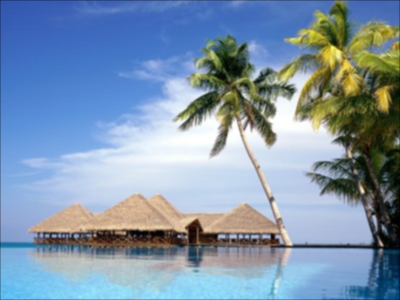
\includegraphics[scale=0.5]{output/p1-2-1-0}}
		}
	}
	\quad
	\subfloat[(\textbf{p1-2-1-1})]{
		{
			\setlength{\fboxsep}{1pt}
			\setlength{\fboxrule}{1pt}
			\fbox{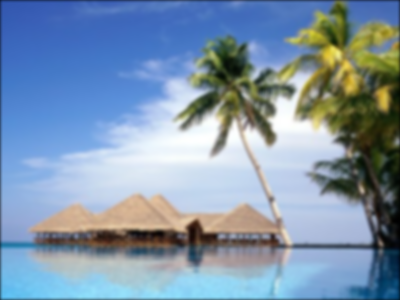
\includegraphics[scale=0.5]{output/p1-2-1-1}}
		}
	}
	\quad
	\subfloat[(\textbf{p1-2-1-2})]{
		{
			\setlength{\fboxsep}{1pt}
			\setlength{\fboxrule}{1pt}
			\fbox{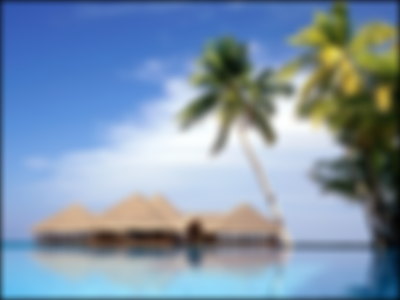
\includegraphics[scale=0.5]{output/p1-2-1-2}}
		}
	}
	\caption{Images (a), (b) and (c) are the result of the convolution with gaussian masks, respectively 3x3, 7x7 and 15x15}
	\label{fig:convolution}
\end{figure}

\begin{table}[!h]
 \centering
 \begin{tabular}{|c|c|c|c|}
	\hline
		& \multicolumn{3}{c|}{\textbf{Time (ms)}} \\ \hline
		\backslashbox{\textbf{Convolution}}{\textbf{Mask Size}}    & \textbf{3x3}         & \textbf{7x7}          & \textbf{15x15}      \\ \hline
	\textbf{Implemented}  & 5.123      & 4.8681      & 5.238     \\ \hline
	\textbf{OpenCV} & 0.006      & 0.004       & 0.019     \\ \hline
	\end{tabular}
 \caption{Comparission of time between our implementation and OpenCV convolution.}
 \label{table:convolution-opencv}
 \end{table}

\textbf{2.2 )} To store the gaussian and laplacian pyramids of this project we chose a list, in which each node of it holds a level of the pyramid. Since the data structure is a list the access method is as in a array, $pyramid[i]$ returns the image in the ith pyramid level, disregarding then, the necessity to implement an access function. The strategy chosen to implement the interpolation was the bilinear interpolation. These decisions were taken regarding the time to implement and simplicity to understand. It is also worth noting that due to some confusion about the meaning of Up and Down, these functions were renamed as follow: Expand referring to the action of expand the image width and height, and Contract analogously. Figure \ref{fig:gaussianPyramid} shows the pyramid formed with the implemented function. \\

\begin{figure}[!h]
	\centering
	\subfloat[(\textbf{p1-2-2-0})]{
		{
			\setlength{\fboxsep}{1pt}
			\setlength{\fboxrule}{1pt}
			\fbox{
\includegraphics[scale=0.75]{output/p1-2-2-0}}
		}
	}
	\quad
	\subfloat[(\textbf{p1-2-2-1})]{
		{
			\setlength{\fboxsep}{1pt}
			\setlength{\fboxrule}{1pt}
			\fbox{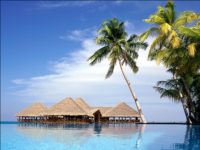
\includegraphics[scale=0.75]{output/p1-2-2-1}}
		}
	}
	\quad
	\subfloat[(\textbf{p1-2-2-2})]{
		{
			\setlength{\fboxsep}{1pt}
			\setlength{\fboxrule}{1pt}
			\fbox{
\includegraphics[scale=0.75]{output/p1-2-2-2}}
		}
	}
	\caption{Images (a), (b) and (c) composing the Gaussian Pyramid formed from image \textbf{p1-1-0}}
	\label{fig:gaussianPyramid}
\end{figure}

\textbf{2.3 )} The laplacian pyramid demanded more attention to its details, such as the fact that the last level of the pyramid is a copy of the same level at the gaussian pyramid. This particular level is used to perform the reconstruction of the original image, first the image is extended and interpolated, to match the previous level size, then it is summed with the previous level of the pyramid, the repetition of these steps result in the original image that was compressed in the pyramid, Figure \ref{fig:placePyramid} shows the laplacian pyramid. \\

\begin{figure}[!h]
	\centering
	\subfloat[(\textbf{p1-2-3-0})]{
		{
			\setlength{\fboxsep}{1pt}
			\setlength{\fboxrule}{1pt}
			\fbox{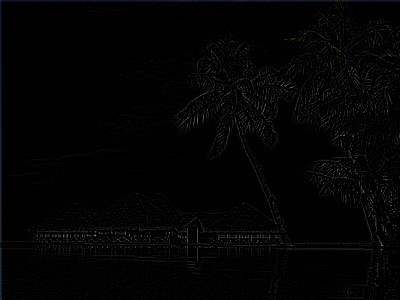
\includegraphics[scale=0.75]{output/p1-2-3-0}}
		}
	}
	\quad
	\subfloat[(\textbf{p1-2-3-1})]{
		{
			\setlength{\fboxsep}{1pt}
			\setlength{\fboxrule}{1pt}
			\fbox{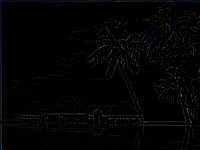
\includegraphics[scale=0.75]{output/p1-2-3-1}}
		}
	}
	\quad
	\subfloat[(\textbf{p1-2-3-2})]{
		{
			\setlength{\fboxsep}{1pt}
			\setlength{\fboxrule}{1pt}
			\fbox{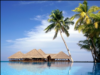
\includegraphics[scale=0.75]{output/p1-2-3-2}}
		}
	}
	\caption{Images (a), (b) and (c) composing the LaPlacian Pyramid formed from image \textbf{p1-1-0}}
	\label{fig:placePyramid}
\end{figure}


\textbf{2.4 )} The process of blending two images implement here is referred as "Splining Regions of Arbitrary Shape" in Burt and Adelson's paper, it consists of three gaussian pyramids $GA$, $GB$ and $GM$, and three laplacian pyramids $LA$, $LB$ and $LS$, in which $LS$ is the resulting pyramid and the image at its base is the blended image. The algorithm to blend the images uses both $LA$, $LB$ and $GM$ pyramids simultaneously, from their top it multiply each lower resolution image with the equivalent mask (Figure \ref{fig:blendingProcess} (a) and (b)), sum the resulting images with each other (Figure \ref{fig:blendingProcess} (c)) and expand the resulting image, repeat these steps and the resulting image at the base of $LS$ is the blended image. The core point of this process is the gaussian filter applied to the mask that smooth its borders and the expand operation performed in the pyramid. Two tests were performed reproducing the original results, in Figure \ref{fig:blending} (a) and (b) were merged using Figure \ref{fig:blending} (c) as mask and Figure \ref{fig:blendingFurther} (a) and (b) were merged using Figure \ref{fig:blendingFurther} (c) as mask, resulting in Figure \ref{fig:blendingResult} (b).

\begin{figure}[!h]
	\centering
	\subfloat[(\textbf{report-p1-2-4-0})]{
		{
			\setlength{\fboxsep}{1pt}
			\setlength{\fboxrule}{1pt}
			\fbox{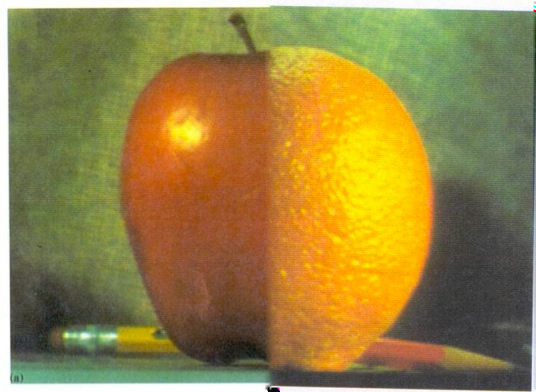
\includegraphics[scale=1]{output/p1-2-4-0}}
		}
	}
	\quad
	\subfloat[(\textbf{report-p1-2-4-1})]{
		{
			\setlength{\fboxsep}{1pt}
			\setlength{\fboxrule}{1pt}
			\fbox{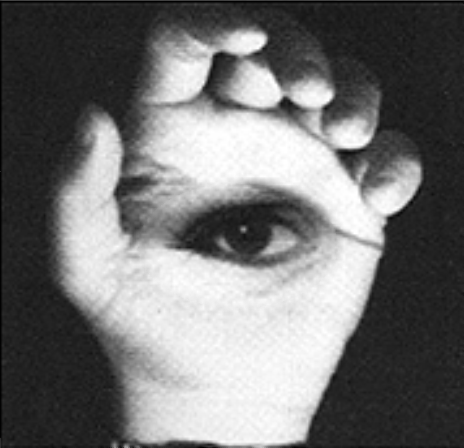
\includegraphics[scale=1]{output/p1-2-4-1}}
		}
	}
	\quad
	\subfloat[(\textbf{report-p1-2-4-2})]{
		{
			\setlength{\fboxsep}{1pt}
			\setlength{\fboxrule}{1pt}
			\fbox{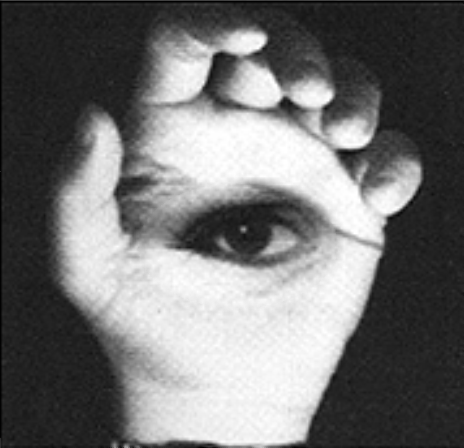
\includegraphics[scale=1]{output/p1-2-4-1}}
		}
	}
	\caption{Images (a) and (b) are the result of the blending operation.}
	\label{fig:blendingProcess}
\end{figure}

\begin{figure}[!h]
	\centering
	\subfloat[(\textbf{p1-2-4-3})]{
		{
			\setlength{\fboxsep}{1pt}
			\setlength{\fboxrule}{1pt}
			\fbox{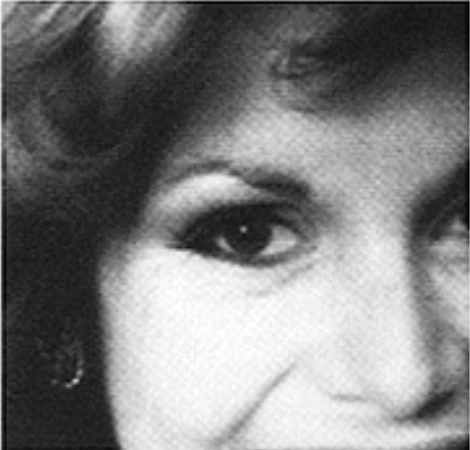
\includegraphics[scale=0.25]{input/p1-2-4-3}}
		}
	}
	\quad
	\subfloat[(\textbf{p1-2-4-4})]{
		{
			\setlength{\fboxsep}{1pt}
			\setlength{\fboxrule}{1pt}
			\fbox{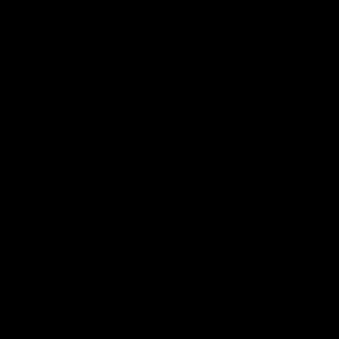
\includegraphics[scale=0.25]{input/p1-2-4-4}}
		}
	}
	\quad
	\subfloat[(\textbf{p1-2-4-5})]{
		{
			\setlength{\fboxsep}{1pt}
			\setlength{\fboxrule}{1pt}
			\fbox{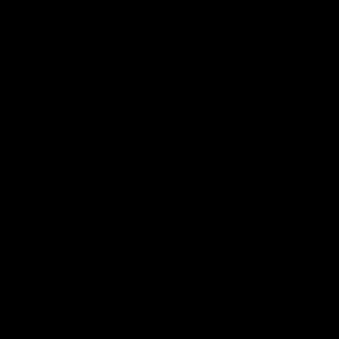
\includegraphics[scale=0.25]{input/p1-2-4-5}}
		}
	}
	\caption{Images (a), (b) and (c) used for further testing the blending operations.}
	\label{fig:blendingFurther}
\end{figure}

\begin{figure}[!h]
	\centering
	\subfloat[(\textbf{p1-2-4-0})]{
		{
			\setlength{\fboxsep}{1pt}
			\setlength{\fboxrule}{1pt}
			\fbox{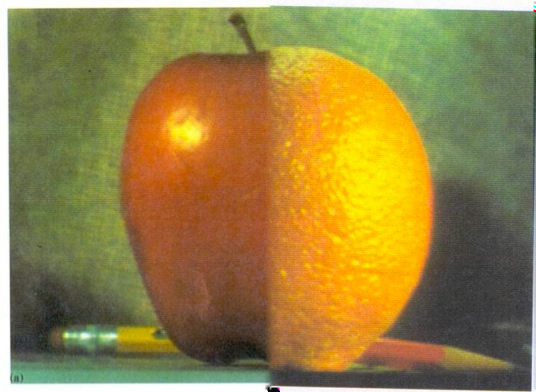
\includegraphics[scale=0.25]{output/p1-2-4-0}}
		}
	}
	\quad
	\subfloat[(\textbf{p1-2-4-1})]{
		{
			\setlength{\fboxsep}{1pt}
			\setlength{\fboxrule}{1pt}
			\fbox{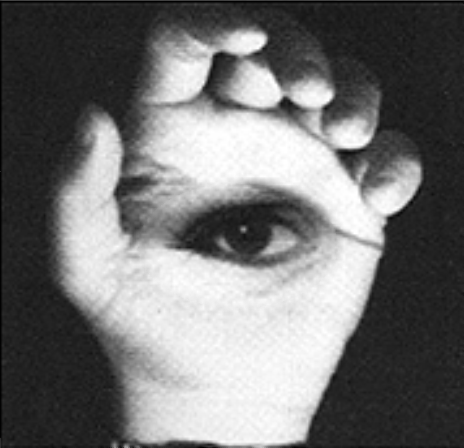
\includegraphics[scale=0.25]{output/p1-2-4-1}}
		}
	}
	\caption{Images (a) and (b) are the result of the blending operation.}
	\label{fig:blendingResult}
\end{figure}

\newpage

\textbf{\LARGE Question 3 - Frequency Blending} \\

In this question, we will present some experiments developed using \emph{numpy} and \emph{OpenCV} function in order to transform the image from the spatial domain to the frequency domain. The process will be divided into two different experiments. \\

On the first one (\textbf{3.1}), we will use the transformation and make some modifications to the phase and magnitude in order to see the impact on the image recontructed. On the second experiment (\textbf{3.2}), we will be blending the two images used into the question \textbf{4.2} in order to check how it is compared to the spatial blending. \\

\textbf{3.1 )} Exploring Fourier Space \\

In order to explore the fourier space, we implemented two functions. One to transform an image into magnitude and phase, and the other to reconstruct the image from magnitude and phase. The Figure \ref{fig:mag-phase} shows the magnitude and phase obtained transforming the Figure \ref{fig:p1-1-0} to the frequency domain. \\

\begin{figure}[!h]
	\centering
	\subfloat[(\textbf{p1-3-1-0})]{
		{
			\setlength{\fboxsep}{1pt}
			\setlength{\fboxrule}{1pt}
			\fbox{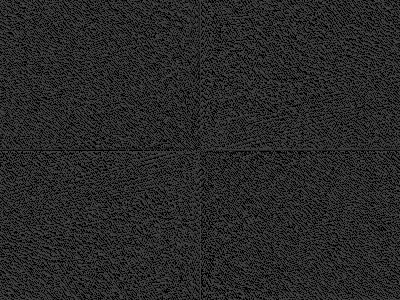
\includegraphics[scale=0.5]{output/p1-3-1-0}}
		}
		\label{fig:phase}
	}
	\quad
	\subfloat[(\textbf{p1-3-1-1})]{
		{
			\setlength{\fboxsep}{1pt}
			\setlength{\fboxrule}{1pt}
			\fbox{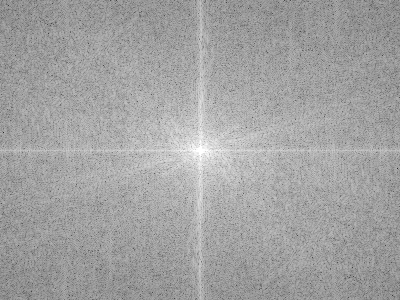
\includegraphics[scale=0.5]{output/p1-3-1-1}}
		}
		\label{fig:magnitude}
	}
	\caption{(a) Phase and (b) Magnitude images created on the fourier transform using image \textbf{p0-1-0}.}
	\label{fig:mag-phase}
\end{figure}

In order to create these images, the results of the fourier transform were shifted to the center and then reduced by the functions, $20*log_e(magnitude)$ and $40*log_e(phase)$. These values were used to mantain the values between 0 and 255, which could be showed as an image. These values are translated back when doing the reverse of the fourier transform. \\

The Figure \ref{fig:phase} shows the phase of the image, it is hard to obtain some information from this image. However, it is respective to the directions of the image. Moreover, the Figure \ref{fig:fig:magnitude} shows the values to the magnitude, the intensity shows the values of the magnitude. In both Figures, light pixels indicates high values.

We can have a little more information with the magnitude image, it is noticeably that the image is bright which indicates that the image on Figure \ref{fig:p0-1-0} has more high frequency than low frequencies. \\

In the next experiments, we will be changing the values of the phase and magnitude images before doing the reverse of Fourier transform. This process should reconstruct the original image, we will be changing the images by percentages. So, in every experiment this process was made using 1 pixel, 25\%, 50\%, 75\% and 100\% of the pixels from the phase or magnitude image.

This pixels might be extract in two different ways, greatest or lowest (e.g. 25\% lowest pixels on phase image). In the image reconstruct using 100\% of the pixels all the images were perfectly reconstruct, a effect which was expected (Figure \ref{fig:inverse}). All the following experiments were made using the Figure \ref{fig:p1-1-0} in grayscale, the grayscale was used for more simplicity and further on one experiment will show the results in a colored image.


\begin{figure}[!h]
	\centering
	{%
		\setlength{\fboxsep}{1pt}%
		\setlength{\fboxrule}{1pt}%
		\fbox{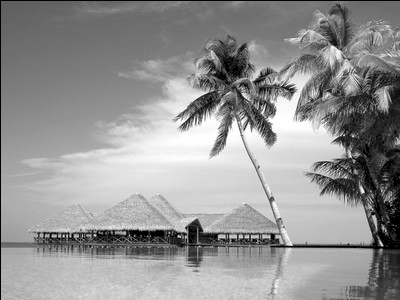
\includegraphics[scale=0.55]{output/p1-3-1-6}}%
	}%
	\caption{Reconstructed image after inverse Fourier transform using 100\% of pixels in magnitude and phase images. (\textbf{p1-3-1-6, p1-3-1-11, p1-3-1-16, and p1-3-1-21})}
	\label{fig:inverse}
\end{figure}


In order to show the differences when changing the phase or magnitude image, we will divide the experiments into two parts:

\begin{itemize}
	\item \textbf{Phase} - First we will be changing the phase image and performing the inverse of Fourier. In this experiment we were expecting to the position of the objects on the image to move. The Figure \ref{fig:phaseINC} show the results when using only the lowest values of the phase image.

	\begin{figure}[!h]
		\centering
		\subfloat[Only lowest pixel (\textbf{p1-3-1-2})]{
			{
				\setlength{\fboxsep}{1pt}
				\setlength{\fboxrule}{1pt}
				\fbox{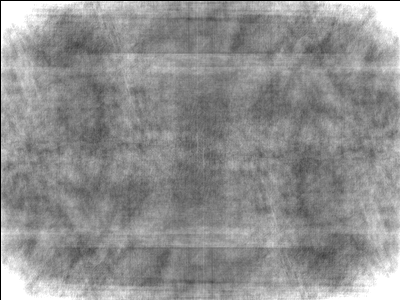
\includegraphics[scale=0.4]{output/p1-3-1-2}}
			}
			\label{fig:phaseinc1}
		}
		\quad
		\subfloat[Lowest 25\% (\textbf{p1-3-1-3})]{
			{
				\setlength{\fboxsep}{1pt}
				\setlength{\fboxrule}{1pt}
				\fbox{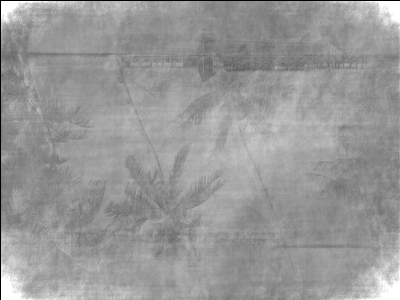
\includegraphics[scale=0.4]{output/p1-3-1-3}}
			}
			\label{fig:phaseinc25}
		}
		\quad
		\subfloat[Lowest 50\% (\textbf{p1-3-1-4})]{
			{
				\setlength{\fboxsep}{1pt}
				\setlength{\fboxrule}{1pt}
				\fbox{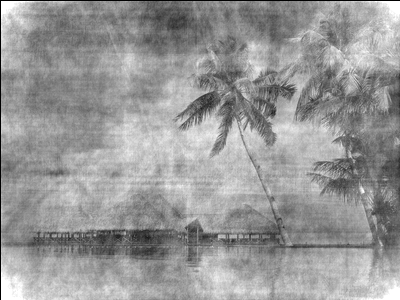
\includegraphics[scale=0.4]{output/p1-3-1-4}}
			}
			\label{fig:phaseinc50}
		}
		\quad
		\subfloat[Lowest 75\% (\textbf{p1-3-1-5})]{
			{
				\setlength{\fboxsep}{1pt}
				\setlength{\fboxrule}{1pt}
				\fbox{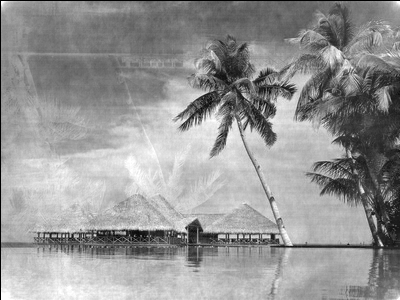
\includegraphics[scale=0.4]{output/p1-3-1-5}}
			}
			\label{fig:phaseinc75}
		}
		
		\caption{Results of inverse Fourier transform using the lowest values on the phase image.}
		\label{fig:phaseINC}
	\end{figure}
	
	As we can see, the image shows us information about the orientation of the image. In this way, selecting different values changes the orientation of the image. Another interesting fact is the upside down elements, which occurs because of the range in which the transform is working, from 0 to 380 degrees.
	
	In other hand, the Figure \ref{fig:phaseDESC} shows the results when using the highest values to the phase image.
	
	\begin{figure}[!h]
		\centering
		\subfloat[Only highest pixel (\textbf{p1-3-1-7})]{
			{
				\setlength{\fboxsep}{1pt}
				\setlength{\fboxrule}{1pt}
				\fbox{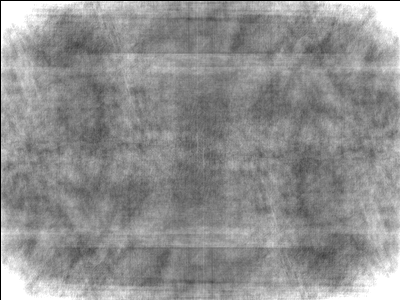
\includegraphics[scale=0.4]{output/p1-3-1-7}}
			}
			\label{fig:phasedesc1}
		}
		\quad
		\subfloat[Highest 25\% (\textbf{p1-3-1-8})]{
			{
				\setlength{\fboxsep}{1pt}
				\setlength{\fboxrule}{1pt}
				\fbox{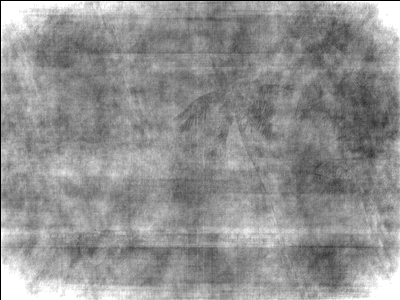
\includegraphics[scale=0.4]{output/p1-3-1-8}}
			}
			\label{fig:phasedesc25}
		}
		\quad
		\subfloat[Highest 50\% (\textbf{p1-3-1-9})]{
			{
				\setlength{\fboxsep}{1pt}
				\setlength{\fboxrule}{1pt}
				\fbox{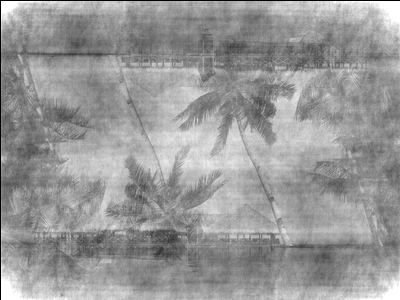
\includegraphics[scale=0.4]{output/p1-3-1-9}}
			}
			\label{fig:phasedesc50}
		}
		\quad
		\subfloat[Highest 75\% (\textbf{p1-3-1-10})]{
			{
				\setlength{\fboxsep}{1pt}
				\setlength{\fboxrule}{1pt}
				\fbox{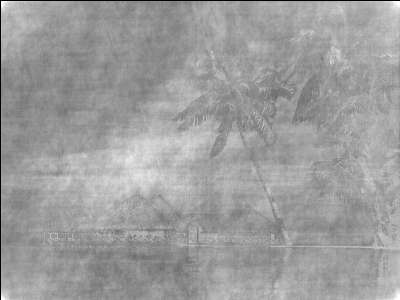
\includegraphics[scale=0.4]{output/p1-3-1-10}}
			}
			\label{fig:phasedesc75}
		}
		
		\caption{Results of inverse Fourier transform using the greatest values on the phase image.}
		\label{fig:phaseDESC}
	\end{figure}
	
	An interesting feature is that the images contain complement information, as example the Figure \ref{fig:phasedesc25} has less information than Figure \ref{fig:phaseinc75}, which completes the information missing on the first image. The same effect might be seen in the other images.
	
	\item \textbf{Magnitude} -  In this part, we will be doing similar experiments, but this time, changing the magnitude image. In this part, we expect to see different results on the intensity of the image, which is described by the magnitude on the frequency domain. The Figure \ref{fig:magnitude} shows the different images obtained on the inverse Fourier transform.
	
	\begin{figure}[!h]
		\centering
		\subfloat[Only lowest pixel (\textbf{p1-3-1-12})]{
			{
				\setlength{\fboxsep}{1pt}
				\setlength{\fboxrule}{1pt}
				\fbox{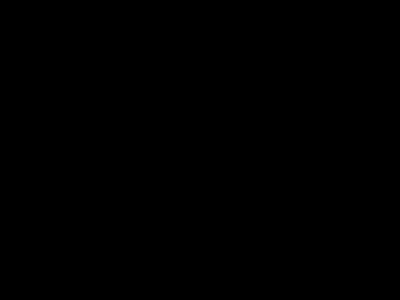
\includegraphics[scale=0.3]{output/p1-3-1-12}}
			}
			\label{fig:magnitudeinc1}
		}
		\quad
		\subfloat[Lowest 25\% (\textbf{p1-3-1-13})]{
			{
				\setlength{\fboxsep}{1pt}
				\setlength{\fboxrule}{1pt}
				\fbox{
\includegraphics[scale=0.3]{output/p1-3-1-13}}
			}
			\label{fig:magnitudeinc25}
		}
		\quad
		\subfloat[Lowest 50\% (\textbf{p1-3-1-14})]{
			{
				\setlength{\fboxsep}{1pt}
				\setlength{\fboxrule}{1pt}
				\fbox{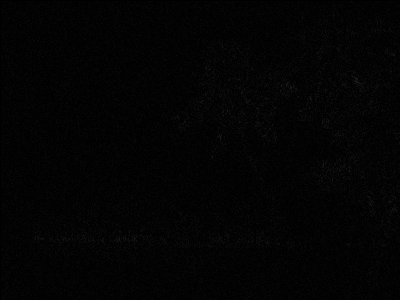
\includegraphics[scale=0.3]{output/p1-3-1-14}}
			}
			\label{fig:magnitudeinc50}
		}
		\quad
		\subfloat[Lowest 75\% (\textbf{p1-3-1-15})]{
			{
				\setlength{\fboxsep}{1pt}
				\setlength{\fboxrule}{1pt}
				\fbox{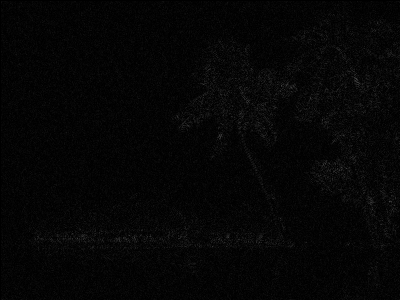
\includegraphics[scale=0.5]{output/p1-3-1-15}}
			}
			\label{fig:magnitudeinc75}
		}
		
		\caption{Results of inverse Fourier transform using the lowest values on the magnitude image.}
		\label{fig:magnitudeINC}
	\end{figure}
		
	By doing this operation, we are using only the low frequency pixels from the image. The first row on image is almost all black pixels, the reason for that is the high frequency on the image used. However, we can see some of the contours being marked in Figure \ref{fig:magnitudeinc75}. This effect produces a image similar to the convolved image on Figure \ref{fig:conv}, which is a High-Pass-Filter. Moreover, The Figure \ref{fig:magnitudeDESC} show the same process using the high frequency on the magnitude.
	
	\begin{figure}[!h]
		\centering
		\subfloat[Only highest pixel (\textbf{p1-3-1-17})]{
			{
				\setlength{\fboxsep}{1pt}
				\setlength{\fboxrule}{1pt}
				\fbox{
\includegraphics[scale=0.5]{output/p1-3-1-17}}
			}
			\label{fig:magnitudedesc1}
		}
		\quad
		\subfloat[Highest 25\% (\textbf{p1-3-1-18})]{
			{
				\setlength{\fboxsep}{1pt}
				\setlength{\fboxrule}{1pt}
				\fbox{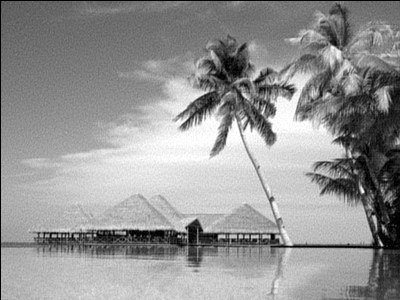
\includegraphics[scale=0.5]{output/p1-3-1-18}}
			}
			\label{fig:magnitudedesc25}
		}
		\quad
		\subfloat[Highest 50\% (\textbf{p1-3-1-19})]{
			{
				\setlength{\fboxsep}{1pt}
				\setlength{\fboxrule}{1pt}
				\fbox{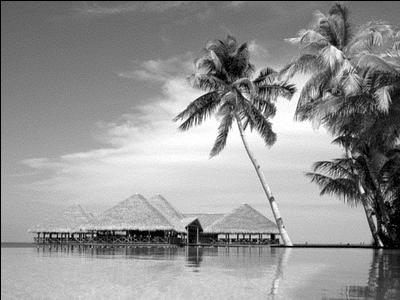
\includegraphics[scale=0.5]{output/p1-3-1-19}}
			}
			\label{fig:magnitudedesc50}
		}
		\quad
		\subfloat[Highest 75\% (\textbf{p1-3-1-20})]{
			{
				\setlength{\fboxsep}{1pt}
				\setlength{\fboxrule}{1pt}
				\fbox{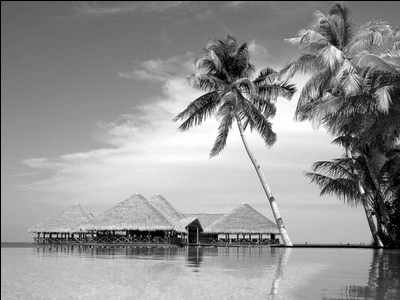
\includegraphics[scale=0.5]{output/p1-3-1-20}}
			}
			\label{fig:magnitudedesc75}
		}
		
		\caption{Results of inverse Fourier transform using the highest values on the magnitude image.}
		\label{fig:magnitudeDESC}
	\end{figure}
	
	As we would expect, the high frequencies on the image were maintained. So, even the using only 25\% of the pixels on magnitude image the reconstructed image is really good. We can note that the quality of the reconstructed image is proportional with the percentage used on the magnitude image. The first image (Figure \ref{fig:magnitudedesc1}) does not have enough information to reconstruct the image, but the color information is showing the predominant color intensity (with just the highest pixel).
	
\end{itemize}

\newpage

In order to show that our implementation could be used with colored images, we used same experiment as before. The Figure \ref{fig:magnitudeDESCColored} shows the result of using the highest values on the magnitude image on a colored image.\\


\begin{figure}[!h]
	\centering
	\subfloat[Only highest pixel (\textbf{p1-3-1-22})]{
		{
			\setlength{\fboxsep}{1pt}
			\setlength{\fboxrule}{1pt}
			\fbox{
\includegraphics[scale=0.5]{output/p1-3-1-22}}
		}
		\label{fig:magnitudedesc1}
	}
	\quad
	\subfloat[Highest 25\% (\textbf{p1-3-1-23})]{
		{
			\setlength{\fboxsep}{1pt}
			\setlength{\fboxrule}{1pt}
			\fbox{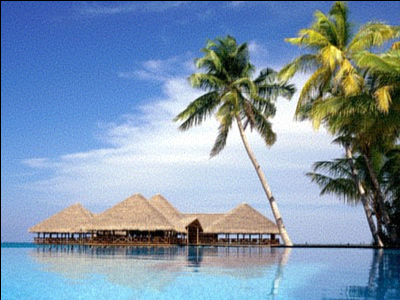
\includegraphics[scale=0.5]{output/p1-3-1-23}}
		}
		\label{fig:magnitudedesc25}
	}
	\quad
	\subfloat[Highest 50\% (\textbf{p1-3-1-24})]{
		{
			\setlength{\fboxsep}{1pt}
			\setlength{\fboxrule}{1pt}
			\fbox{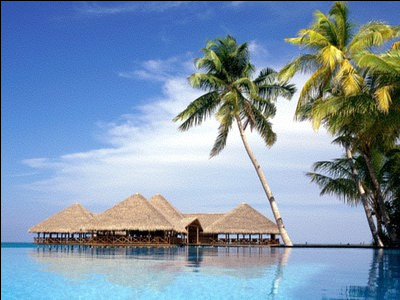
\includegraphics[scale=0.5]{output/p1-3-1-24}}
		}
		\label{fig:magnitudedesc50}
	}
	\quad
	\subfloat[Highest 75\% (\textbf{p1-3-1-25})]{
		{
			\setlength{\fboxsep}{1pt}
			\setlength{\fboxrule}{1pt}
			\fbox{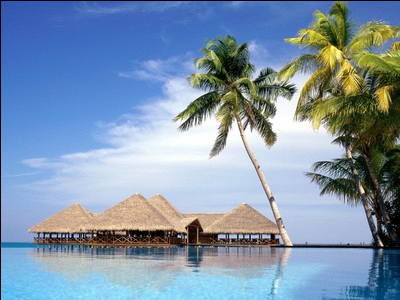
\includegraphics[scale=0.5]{output/p1-3-1-25}}
		}
		\label{fig:magnitudedesc75}
	}
	\quad
	\subfloat[Highest 100\% (\textbf{p1-3-1-26})]{
		{
			\setlength{\fboxsep}{1pt}
			\setlength{\fboxrule}{1pt}
			\fbox{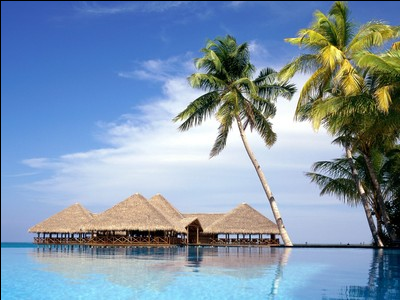
\includegraphics[scale=0.5]{output/p1-3-1-26}}
		}
		\label{fig:magnitudedesc100}
	}
	
	\caption{Results of inverse Fourier transform using the highest values on the magnitude image using colored images.}
	\label{fig:magnitudeDESCColored}
\end{figure}

In order to use a colored image, the Fourier transformation was processed three times, one for each color channel. Note that the Figure \ref{fig:magnitudedesc100} is the reconstruction of the Figure \ref{fig:p1-1-0}, which indicates that the process of the Fourier transform was successfull.

\newpage

\textbf{3.2 )} Blending \\

In order to do the blending on the frequency domain, we first transformed both images from spatial to frequency domain, using Fourier transform. After this, we have two vectors for each image representing the magnitude and phase values. Our first approach was to sum the vectors together, this approach obviously did not work (Figure \ref{fig:fourier1}). The phase vector, responsible to the imaginary part (on polar coordinates), could not be summed in this way, the reason is we would lose information. \\

\begin{figure}[!h]
	\centering
	{%
		\setlength{\fboxsep}{1pt}%
		\setlength{\fboxrule}{1pt}%
		\fbox{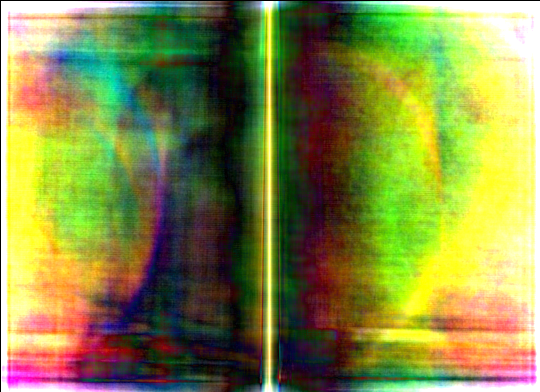
\includegraphics[scale=0.5]{report/Fourier.png}}%
	}%
	\caption{Blending adding phase and magnitude vectors.}
	\label{fig:fourier1}
\end{figure}

After this approach, we have tried to implement the blending using a different values for the images into the magnitude as phase. As example: we would get 50\% of highest values of both images and them sum them up. We were expecting that the sum of the zeros, inserted on the 50\% lowest values, would work using a certain mask. This approach was not a disaster, but it still a bad blending over all (Figure \ref{fig:fourier2}). \\

\begin{figure}[!h]
	\centering
	{%
		\setlength{\fboxsep}{1pt}%
		\setlength{\fboxrule}{1pt}%
		\fbox{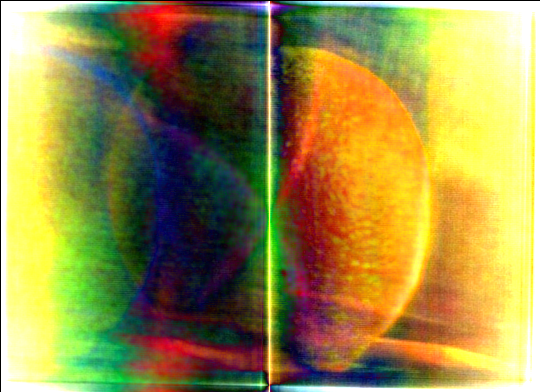
\includegraphics[scale=0.5]{report/Fourier50.png}}%
	}%
	\caption{Blending adding phase and magnitude vectors using only 50\% highest values.}
	\label{fig:fourier2}
\end{figure}

Also these tries, we started thinking about our results. Our conclusion was that no merging between the phase and magnitude would work as a blending, moreover, we concluded that our approach was not working as expected. Looking at the images we could see that a great number of information was being lost, even just adding them or trying to use a mixture of pixels from magnitude and phase. \\

After some thinking, we figure it that the summation should work. However, we were dealing with complex numbers and we were adding the phase as it was a normal number. In order to fix it, we first construct a \emph{numpy} complex function using $magnitude * np.exp(1j*phase)$, in which $magnitude$ and $phase$ are vectors. After creating one function for each image, we were able to sum them up, which the \emph{numpy} would do using the correct complex summation. The Figure \ref{fig:blending} shows the result of this process.

\begin{figure}[!h]
	\centering
	{%
		\setlength{\fboxsep}{1pt}%
		\setlength{\fboxrule}{1pt}%
		\fbox{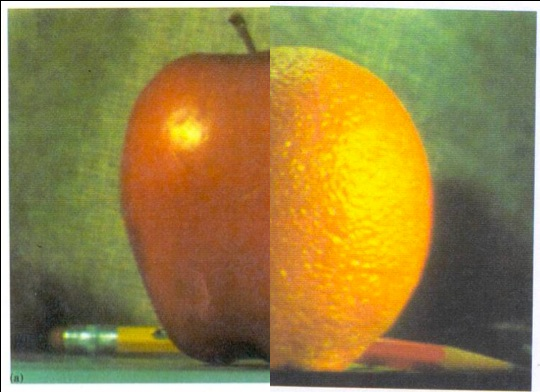
\includegraphics[scale=0.5]{output/p1-3-2-0.png}}%
	}%
	\caption{Blended image using the \emph{numpy} summation of complex numbers.}
	\label{fig:fourier2}
\end{figure}

The generated image is a blend of two images, but if it is compared to the blending generated using pyramids (Figure \ref{fig:aksda}) the contrast of the images are too high. After that some filtering approaches were tried to solve the contrast, but nothing gave a better result. \\

We then tried to use the pyramids with the frequency domain, but we had problem with the up sampling and down sampling. Because we could not change pixels arbitrary, mainly because one pixel on frequency domain represents more information from the image, as seen in exercise \emph{\textbf{3.1} Exploring Fourier Space}. We did not have enough time to explore more this blending, but our intuition is that it might be possible if some ``tricks'' are applied to the frequency domain in order to blend the images. 

\end{document}
